\documentclass[letterpaper,11pt]{article}
\usepackage[spanish]{babel}
\usepackage[utf8]{inputenc}
\usepackage[T1]{fontenc}
\usepackage{graphicx}
\usepackage{geometry}
\usepackage{array,longtable,booktabs}
\usepackage{setspace}
\usepackage{titlesec}
\usepackage[shortlabels]{enumitem}
\usepackage{amsmath,amssymb,amsfonts,amsthm}
\usepackage{float}
\usepackage{xcolor}
\usepackage{realboxes}
\usepackage{fancyhdr}
\usepackage{anysize}
\usepackage{hyperref}
\usepackage{verbatim}
\usepackage{icomma}
\usepackage{tikz}
\usepackage{pgfplots}
\usepackage{framed}
\usetikzlibrary{arrows,decorations.fractals,decorations.pathmorphing,shadows}
\pgfplotsset{compat=1.18}
\geometry{margin=2.5cm}
\definecolor{lightgrey}{rgb}{0.95,0.95,0.95}
\newcommand{\code}[1]{\Colorbox{lightgrey}{\texttt{#1}}}
\newcommand{\s}{\vspace{0.2cm}}
\newcommand{\R}{{\mathbb R}}
\newcommand{\C}{{\mathbb C}}
\newcommand{\Z}{\mathbb{Z}}
\newcommand{\N}{{\mathbb N}}
\newcommand{\ds}{\displaystyle}
\newcommand{\sen}{\mathop{\rm sen}\nolimits}
\newcommand{\n}{\noindent}
\newcommand{\ex}{\mathop{\rm e}\nolimits}
\newcommand{\ssi}{\Longleftrightarrow}
\newcommand{\implica}{\Longrightarrow}
\DeclareMathOperator{\var}{Var}
\DeclareMathOperator{\cov}{Cov}
\DeclareMathOperator{\Exp}{\mathbb{E}}
\newcommand{\E}[1]{\Exp\left[#1\right]}
\DeclareMathOperator{\plim}{plim}
\DeclareMathOperator{\Prob}{\mathbb{P}}
\newcommand{\prob}[1]{\Prob\left(#1\right)}
\newcommand{\abs}[1]{\left|#1\right|}
\newcommand{\pto}{\xrightarrow{p}}
\pagestyle{fancy}
\fancyhf{}
\fancyhead[L]{INGENIERÍA COMERCIAL}
\fancyhead[R]{ICS-294 | II Semestre 2026}
\fancyfoot[C]{\thepage}
\setlength{\headheight}{14pt}
\renewcommand{\headrulewidth}{0.4pt}
\renewcommand{\footrulewidth}{0pt}

\begin{document}
\noindent
\begin{minipage}{0.39\textwidth}
    
\includegraphics[width=0.82\linewidth]{logoUSM.png}
\end{minipage}
\hfill
\begin{minipage}{0.59\textwidth}
    \raggedleft
    \textbf{INGENIERÍA COMERCIAL}\\
    \textbf{2026-2}
\end{minipage}

\vspace{0.4cm}
\hrule
\vspace{0.1cm}
\begin{center}
    {\Large \textbf{Control 3}}\\
    Econometría ICS-294\\
    II Semestre 2026\\
    \vspace{0.3cm}
    Profesor: Francisco Alfaro Medina
\end{center}

\textbf{Instrucciones:}
\begin{itemize}
    \item El trabajo deberá entregarse resuelto a mano.
    \item Cuide la presentación y la redacción de sus respuestas.
    \item Justifique sus respuestas e indique claramente los supuestos y valores críticos utilizados cuando corresponda.
\end{itemize}

\section{Preguntas}
\begin{enumerate}
\item  Con datos de corte transversal de 80 trabajadores, un investigador estima una ecuación de salarios en función de los años de educación ($X_1$), los años de experiencia ($X_2$), los años de antigüedad en la empresa ($X_3$) y las horas trabajadas por semana ($X_4$):
\[
Y_i = \beta_0 + \beta_1 X_{1i} + \beta_2 X_{2i} + \beta_3 X_{3i} + \beta_4 X_{4i} + u_i
\]
Sospecha que la estructura salarial difiere entre el sector público y el sector privado, por lo que estima la regresión por separado para cada grupo y obtiene:

\begin{center}
\begin{tabular}{lcc}
\hline
 & Observaciones & Suma de cuadrados residuales (SSR) \\
\hline
Muestra completa (restringida) & $n = 80$ & $SSR_R = 90$ \\
Submuestra 1 (sector público)  & $n_1 = 40$ & $SSR_1 = 40$ \\
Submuestra 2 (sector privado)  & $n_2 = 40$ & $SSR_2 = 30$ \\
\hline
\end{tabular}
\end{center}

El modelo tiene $k=4$ regresores más la constante (es decir, $k+1=5$ parámetros). Con un nivel de significancia del $5\%$, el valor crítico es $F_{0,05}(5,\,70) = 2{,}35$.

\begin{enumerate}[label=\alph*)]
    \item  Plantee las hipótesis nula y alternativa del test de Chow.
    \item  Calcule el estadístico $F$ de Chow.
    \item  Concluya: ¿difiere la estructura salarial entre ambos sectores?
\end{enumerate}

    \item  ¿Por qué los estadísticos \(t\) y \(F\) utilizados para contrastar hipótesis no son válidos en presencia de heterocedasticidad? ¿Cómo puede solucionarse este problema?

    \item  Considere el siguiente modelo de regresión lineal para explicar la cantidad de goles de un jugador en el mundial:
\[
Goles_i = \beta_0 + \beta_1 IQ_i + \beta_2 Entrenamiento_i + \beta_3 Edad_i + \beta_4 Delantero_i + u_i
\]
donde $IQ$ es el coeficiente intelectual, $Entrenamiento$ son las horas de entrenamiento, $Edad$ es la edad del jugador y $Delantero = 1$ si el jugador es delantero y $0$ en otro caso.

Para detectar multicolinealidad en la variable $Entrenamiento$ se estima la regresión auxiliar:
\[
Entrenamiento_i = \alpha_0 + \alpha_1 IQ_i + \alpha_2 Edad_i + \alpha_3 Delantero_i + w_i
\]
obteniéndose $R^2_{Entrenamiento} = 0.75$.\\

Con este resultado, se puede afirmar que existe multicolinealidad severa sobre dicha variable. Determine la veracidad de la afirmación, planteando la regla de decisión correspondiente y justificando su respuesta.

    \item  Comente las siguientes afirmaciones, \textbf{determinando} si son falsas, verdaderas o inciertas y \textbf{justificando} su respuesta. En caso de una afirmación falsa, provea un contra-ejemplo.

    \begin{enumerate}
        
        \item  Todo estimador consistente es necesariamente insesgado.

        \medskip
        \textit{Hint:}
        Piense en las propiedades asintóticas y en muestra finita de alguno de los siguientes estimadores (uno es suficiente):
        \begin{enumerate}[(i)]
        
        \item El estimador de variables instrumentales $\widehat \beta_1=\frac{\sum\limits_{i=1}^n\left(z_i - \overline z\right)\left(y_i - \overline y\right)}{\sum\limits_{i=1}^n\left(z_i - \overline z \right) \left(x_i - \overline x \right)}$
        para el parámetro de pendiente $\beta_1$ en el regresor endógeno $x$ con instrumento $z$ en el modelo de regresión lineal simple $y = \beta_0 + \beta_1 x + u$ con $\cov{\left( x, u \right)} \neq 0$, $\cov{\left( z, x \right)} \neq 0$ y $\cov{\left( z, u \right)} = 0$.
        Puede usar los resultados
        $\plim \frac{1}{n} \sum\limits_{i=1}^n \left(z_i - \overline z \right) \left(y_i - \overline y\right)=\cov{\left( z, y \right)}$,
        $plim\frac{1}{n}\sum\limits_{i=1}^n \left(z_i - \overline z \right) \left(x_i - \overline x \right)=\cov{\left( z, x \right)}$
        y
        $\E{\sum\limits_{i=1}^n\left(z_i - \overline z\right)\left(y_i - \overline y \right)} /\E{\sum\limits_{i=1}^n \left( z_i - \overline z \right)\left( x_i - \overline x \right)} =\cov{\left( z, y \right)}/\cov{\left( z, x \right)}$ sin necesidad de demostrar.
                
        \item El estimador
        $\widehat \sigma = \sqrt{\frac{1}{n - k - 1}\sum\limits_{i=1}^n\widehat u_i^2}$ para la desviación estándar $\sigma = \sqrt{\E{u^2}}$ del término de error en el modelo de regresión lineal múltiple $y = \boldsymbol{x}'\boldsymbol{\beta} + u$ con $\E{u \mid \boldsymbol{x}} = \boldsymbol{0}$, donde $\lbrace \widehat u_i \rbrace_{i=1}^n$ son los residuos de MCO.
        Puede usar los resultados $\plim \widehat \sigma^2 = \sigma^2$ y $\E{\widehat \sigma^2} = \sigma^2$ sin necesidad de demostrar.
                
            \end{enumerate}

        \item  Todo estimador insesgado es necesariamente consistente.
            
            \medskip
            \textit{Hint:}
                Piense en el estimador $\widehat \mu = y_1$ para la media poblacional $\mu = \E{y}$ de la variable aleatoria $y$, donde $y_1$ es la primera observación de la muestra i.i.d. $\lbrace y_i \rbrace_{i=1}^n$.
    
    \end{enumerate}

    \item  Considere el modelo de regresión lineal simple
        $$y=\beta_0+\beta_1x+u,\quad\E{x u}\neq0
        $$
        y sea $z \in \lbrace 0, 1 \rbrace$ una variable instrumental binaria válida para $x$, tal que $\cov{\left( z, x \right)} \neq 0$ y $\cov{\left( z, u \right)} = 0$.
        \textbf{Muestre} que el estimador de variables instrumentales $\widehat \beta_1$ puede escribirse como
        $$\widehat \beta_1=\frac{\overline y_1 -        \overline y_0}{\overline x_1 - \overline x_0}\text{,}$$
        donde $\overline y_0$ y $\overline x_0$ son los promedios muestrales de $y_i$ y $x_i$ sobre la parte de la muestra con $z_i = 0$, y donde $\overline y_1$ y $\overline x_1$ son los promedios muestrales de $y_i$ y $x_i$ sobre la parte de la muestra con $z_i = 1$. 
        Wald (1940) fue el primero en sugerir este estimador, conocido como \textit{estimador de agrupación}.
        
        \smallskip
        \textit{Hint:}
        Recuerde que, en general, el estimador de variables instrumentales para el parámetro de pendiente en el modelo de regresión lineal simple está dado por
        $$\widehat \beta_1=\frac{\sum\limits_{i=1}^n\left(z_i -     \overline z\right)\left(y_i - \overline y            \right)}{\sum\limits_{i=1}^n \left(z_i - \overline z\right) \left(x_i - \overline x \right)}\text{.}$$
\item La tasa de fertilidad general (\textit{grf}) es el numero de niños nacidos por cada 1.000 mujeres en edad de concebir. Para los años 1913 a 1984, la ecuación:

\[
 grf_t = \beta_0 + \beta_1pe_t + \beta_2ww2 + \beta_3pill_t + u_t
\]


donde, 

\textit{pe}: excención de impuestos promedio\\
\textit{ww2}: valor 1 entre los años 1941 y 1945\\
\textit{pill}: valor 1 para los años 1963 en adelante (año en que se implemento la pildora anticonceptiva)\\


Utilizando los datos de la base de datos \textit{Fertil3}, se obtiene:

\begin{centering}
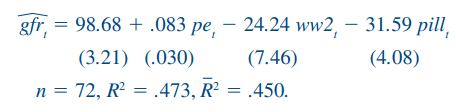
\includegraphics[scale=1.5]{figuras/fertil3.1.png}

\end{centering}

a) ¿Cuales son los efectos de las variables \textit{ww2} y \textit{pills}? ¿son estadisticamente significativos?

Si se añade una tendencia lineal en el tiempo a la ecuación, se obtiene:

\begin{centering}
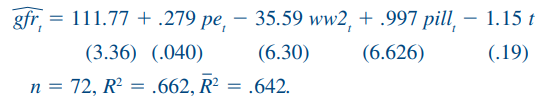
\includegraphics[scale=1.5]{figuras/fertil3.2.png}

\end{centering}

b) ¿Como interpreta el factor de tendencia?

c) ¿cambian los efectos de \textit{ww2} y \textit{pills}?¿siguen siendo significativos?

Ahora añadimos una tendencia cuadratica a la ecuación y obtenemos:

\begin{centering}
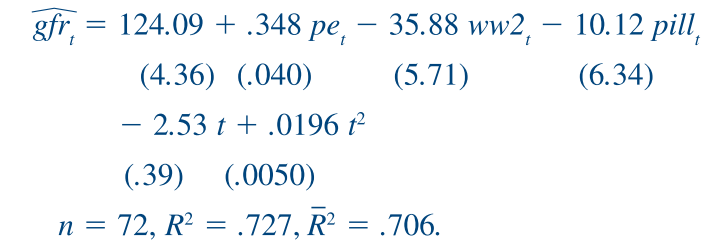
\includegraphics[scale=1]{figuras/fertil3.3.png}

\end{centering}

d) ¿que logra captar esta tendencia cuadratica?

e) ¿será adecuado adicionar una tendencia $t^3$ a nuestro modelo?

\item A partir de la siguiente grafica, responda:

\begin{centering}
    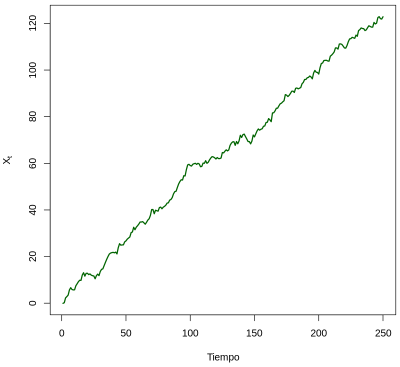
\includegraphics[scale=1]{figuras/Random Walk 1.png}\\
\end{centering}

a) Según sus conocimientos, a partir de la imagen, usted afirmaria que esta serie es ¿estacionaria o tiene raiz unitaria?

b) Plantee el test Dickey-Fuller

c) Ejecute el test de Dickey-Fuller en R, ¿podemos afirmar o no que la serie de tiempo es estacionaria?

Para plantear el test Dickey-Fuller, utilice el siguiente codigo:

\begin{centering}
    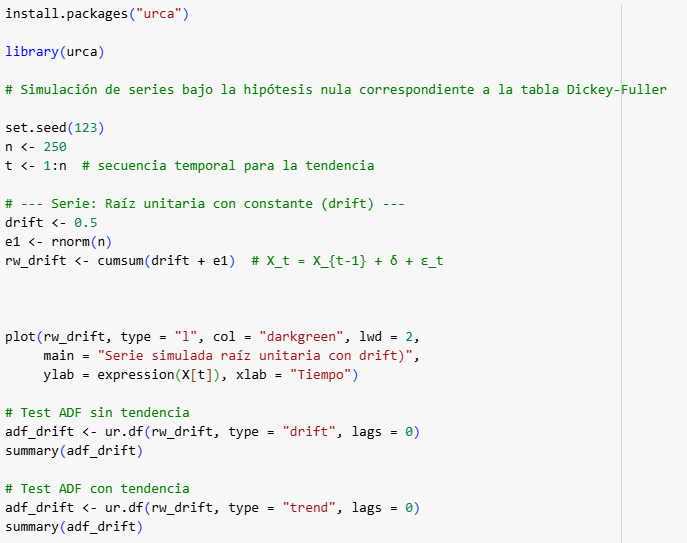
\includegraphics[scale=1]{figuras/Codigo.png}\\
\end{centering}

\item Un investigador ha simulado tres series temporales de 200 observaciones. Dos de ellas corresponden a procesos \textbf{AR(1)} con distintos valores del parámetro \( \phi \), y la tercera corresponde a un proceso de \textbf{ruido blanco} (white noise). Para cada caso se presentan dos gráficos:

\begin{itemize}
    \item A la izquierda: la serie temporal simulada \( \{X_t\} \)
    \item A la derecha: su función de autocorrelación (ACF) hasta el rezago 30
\end{itemize}

Los valores de \( \phi \) utilizados para los procesos AR(1) fueron:

\[
\phi = -0.95 \quad \text{y} \quad \phi = 0.95
\]

\[
X_t = \phi X_{t-1} + \varepsilon_t
\]

Los gráficos han sido rotulados como \textbf{Caso A}, \textbf{Caso B} y \textbf{Caso C} (sin indicar el valor de \( \phi \) ni el tipo de proceso que representan).

\begin{enumerate}
    \item Identifique cuál de los tres casos corresponde al proceso de \textbf{ruido blanco}. Justifique su respuesta con base en el comportamiento de la serie y su ACF.

    \item Para los otros dos casos, asigne a cada uno el valor de \( \phi \) correspondiente. Justifique su elección explicando cómo el signo y la magnitud de \( \phi \) se reflejan en la dinámica de la serie y en la forma de su ACF.

\end{enumerate}

\begin{figure}[H]
    \centering
    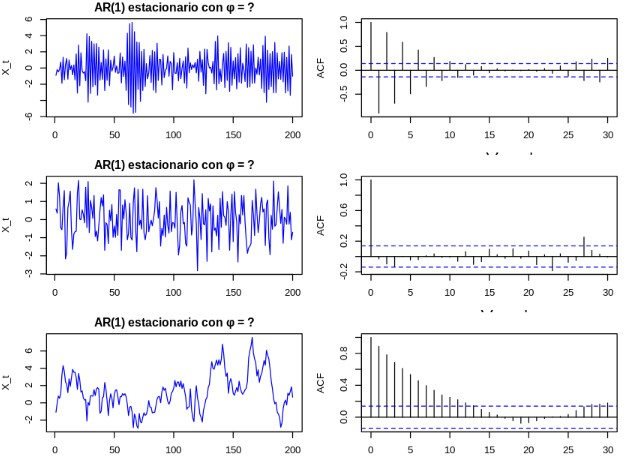
\includegraphics[width=0.7\linewidth]{figuras/autocorr.jpg}
\end{figure}

\item A partir de la bases de datos \textit{hprice1} se realiza la siguiente regresión:

\begin{centering}
    $$price = \beta_0 + \beta_1 bdrms + \beta_2 lotsize + \beta_3sqrft$$
\end{centering}

\textit{bdrms:} número de habitaciones
\textit{lotsize:} tamaño del terreno
\textit{sqrtft:} metros cuadrados construidos

a) Plantee la hipotesis nula del test de Breusch-Pagan

b) Realizamos el test de Breusch-Pagan el cual nos arroja un \textit{p-value = 0.002782} ¿Que consecuencias trae este resultado? ¿Que recomendaría hacer en este caso?

\vspace{1.5cm}

\item A partir de la base de datos \textit{mlb1} se realiza la siguiente regresión:

\begin{centering}
    $$salary = \beta_0 + \beta_1 teamsal + \beta_2games + \beta_3years + \beta_4atbats$$
\end{centering}

Realizando la regresión en R, nos arrojo los siguientes resultados:

\begin{centering}
    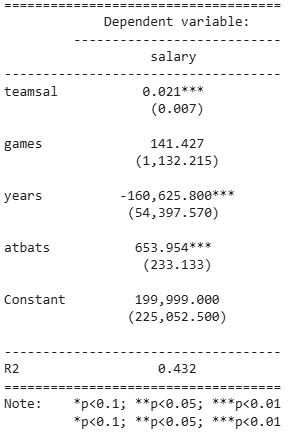
\includegraphics[scale=1]{figuras/mlb1.1.png}\\
\end{centering}

a) plantee una regresión auxiliar que nos permita encontrar multicolinealidad en la variable \textit{games}

b) la regresión auxiliar de \textit{games} nos arrojo $R^2=0.9913$ ¿Cual es el valor del factor de inflación de la varianza? ¿Que se interpreta de este resultado?

c) Utilizando la función \textit{vif} en R, calculamos el factor de variabilidad de la varianza de cada una de las variables y nos arrojo los siguientes valores para cada una:

\begin{itemize}
    \item games: 115.04
    \item teamsal: 1.03
    \item years: 13.77
    \item atbats: 68.92
\end{itemize}

¿Como podría explicar que las variables \textit{games}, \textit{years} y \textit{atbats} resultarán con VIF sobre 10?
¿Cual sería su recomendación?

\item A partir de la base de datos \textit{Attend} se construye la siguiente regresión lineal:

\begin{centering}
    $final = \beta_0 + \beta_1attendrte + \beta_2ACT + \beta_3Soph$
\end{centering}

\begin{centering}
    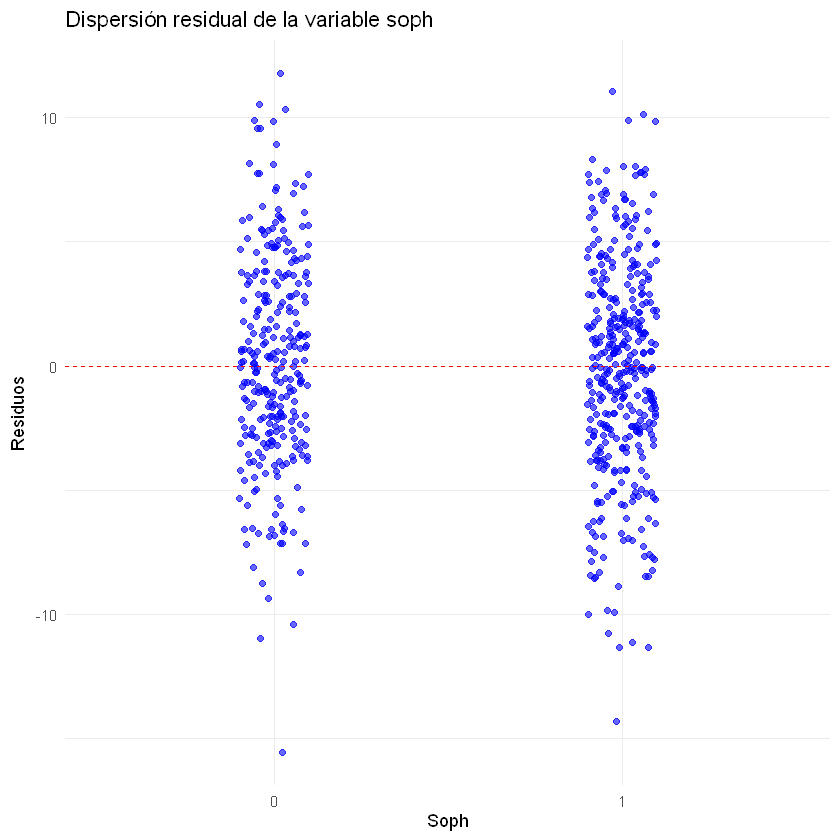
\includegraphics[scale=0.25]{figuras/Shapiro-Wilk.png}\\
\end{centering}

a) a partir de la imagen, ¿se puede afirmar con certeza que los residuos distribuyen normal? ¿se puede afirmar si hay heterocedasticidad u homocedasticidad?

b) Si al realizar el test de Shapiro-Wilk en R nos arroja un \textit{p-value = 0.3619} ¿Que se puede decir de los residuos de la muestra? ¿Que sucederia si \textit{p-value = 0.0001}?

\end{enumerate}

\end{document}
